\documentclass[16pt]{article}
\usepackage[utf8]{inputenc}
\usepackage[russian]{babel}
\usepackage{amsmath}
\usepackage{amssymb}
\usepackage{upgreek}
\usepackage{graphicx}
\usepackage[dvipsnames]{xcolor}
\usepackage{tikz}
\usepackage[export]{adjustbox}                  
\usepackage[hidelinks]{hyperref}

\title {Конспектик по численным методам}
\author {Шоколадные бойцы}

\begin {document}
	\pagenumbering {gobble}
	\maketitle
  
	\newpage 
		\pagenumbering {arabic}
		%1
        Здесь был Игрок
		\section {Понятие погрешности. Абсолютная и относительная погрешности.}	
			Погрешность - отклонение величины от ее истинного значения. То есть, если $a$ реальное значение, а $a^{*}$ приближенное значение, то погрешность будет равна $a-a^{*}$
			\subsection {Причины:}
				\begin {enumerate}
				\item {
					Неустранимая погрешность - 
					$\begin {cases}
						\text{Математическая модель является лишь}\\
						\text{\qquad приближенным описание процеса.}\\
						\text{Исходные данные содержат погрешности.}\\
					\end {cases}$
				}
				\item {Погрершность метода - применяемые методы зачастую являются приближенными.}
				\item {Вычислительная погрешность - при действиях с числами происходит округление.}
				\end {enumerate}
			\subsection {Абсолютная и относительная погрешности}	
				Абсолютная погрешность: $\Delta(a^{*}) = |a-a^{*}|$\\
				Относительная погрешность: $\delta(a^{*}) = \frac{|a-a^{*}|}{|a|} = \frac{\Delta(a^{*})}{|a|}$\\
				Чаще реальное значение неизвестно поэтому используются оценки погрешности.\\
				$\Delta(a^{*}) \leq \overline{\raisebox{3mm}{} \Delta}(a^{*})$,\\
				$\delta(a^{*}) \leq \overline{\raisebox{3mm}{} \delta}(a^{*})$,\\
				где $\overline{\raisebox{3mm}{} \Delta}(a^{*})$ и $\overline{\raisebox{3mm}{} \delta}(a^{*})$ - верхняя граница абсолютной и отностельной погрешности соответственно. При этом если одна из величин известна, вторую можно выразить через нее.
				На практике часто используются следующие приближения:\\
				$\overline{\raisebox{3mm}{}\delta}(a^{*}) \approx \frac{\overline{\raisebox{3mm}{} \Delta}(a^{*})}{|a^{*}|}$,\\				 
				$\overline{\raisebox{3mm}{} \Delta}(a^{*}) \approx |a^{*}| \overline{\raisebox{3mm}{} \delta}(a^{*})$
		%2
		\section {Погрешности арифметических операций и функций.}
			\subsection {Сумма и разность}
				Для абсолютной погрешности:
				Абсолютная погрешность суммы и разности не превосходит суммы абсолютных погрешностей.
				$\Delta(a^{*} \pm b^{*}) \leq \Delta(a^{*}) + \Delta(b^{*})$\\
				Оценка суммы и разности
				$\overline{\raisebox{3mm}{} \Delta}(a^{*} \pm b^{*}) = 
				\overline{\raisebox{3mm}{} \Delta}(a^{*}) + \overline{\raisebox{3mm}{} \Delta}(b^{*})$\\
				Для относительной погрешности:
				Относительная погрешность суммы не превосходит максимальной относительной погрешности.\\
				$\delta (a^{*} + b^{*}) \leq \max(\delta(a^{*}),\delta(b^{*}))$\\
				Относительная погрешность разности выглядит так: \\
				$\delta (a^{*} - b^{*}) \leq \max(\delta(a^{*}),\delta(b^{*})) * \frac{|a+b|}{|a-b|}$\\
				Для оценок относительной погрешности имеем аналогичные неравенства.
			\subsection {Произведение и частное.}
				Для абсолютной погрешности:\\
				Абсолютная погрешность произведения и частного не превышает суммы абсолютных погрешностей.\\
				$\Delta(a^{*} * b^{*}) \leq \Delta(a^{*}) + \Delta(b^{*})$\\
				$\Delta(a^{*} / b^{*}) \leq \Delta(a^{*}) + \Delta(b^{*})$\\
				Оценка произведения и частного:\\
				$\delta(a^{*}*b^{*}) \approx (\overline{\raisebox{3mm}{} \delta}(a^{*}) + \overline{\raisebox{3mm}{} \delta}(b^{*}))*|a^{*}*b^{*}|$\\
				$\delta(a^{*}/b^{*}) \approx (\overline{\raisebox{3mm}{} \delta}(a^{*}) + \overline{\raisebox{3mm}{} \delta}(b^{*}))*|a^{*}/b^{*}|$\\
				Для относительной погрешности:\\
				$\delta (a^{*}b^{*}) \leq \delta(a^{*}) + \delta(b^{*}) + \delta(a^{*})\delta(b^{*})$\\
				$\delta (a^{*}/b^{*}) \leq \frac{\delta(a^{*}) + \delta(b^{*})}{1 - \delta(b^{*})}$\\
				Оценка произведения и частного:\\
				$\overline{\raisebox{3mm}{} \delta}(a^{*}*b^{*}) \approx \overline{\raisebox{3mm}{} \delta}(\frac{a^{*}}{b^{*}}) \approx \overline{\raisebox{3mm}{} \delta}(a^{*}) + \overline{\raisebox{3mm}{} \delta}(b^{*})$
			\subsection {Функции.}
				Пусть $f(x) = f(x_1,\ x_2,\ x_3,\ ...,\ x_m)$ функция от $m$ переменных, дифференцируемая в области G, вычисление которой производится на $x^{*}_1,\ x^{*}_2,\ x^{*}_3,\ ...,\ x^{*}_m$.\\
				\subsubsection{Абсолютная погрешность.}
				$\Delta(y^{*}) \leq \sum_{j=1}^{m} \underset{[x,\ x^{*}]}{max}|f'_{x_j}|\Delta(x^{*}_j)$, где $[x,\ x^{*}]$ отрезок из $x$ d $x^{*}$\\
				Для оценки верно следующее:\\
				$\overline{\raisebox{3mm}{} \Delta}(y^{*})\approx \sum_{j=1}^{m} |f'_{x_j}(x^{*})|\overline{\raisebox{3mm}{} \Delta}(x^{*}_j)$\\
				$\overline{\raisebox{3mm}{} \Delta}(y^{*})\approx \sum_{j=1}^{m} |f'_{x_j}(x)|\overline{\raisebox{3mm}{} \Delta}(x^{*}_j)$\\
				\subsubsection{Относительная погрешность.}
				$\overline{\raisebox{3mm}{} \delta}(y^{*}) \approx \sum_{j=1}^{m} v^{*}_j \overline{\raisebox{3mm}{} \delta}(x^{*}_j)$\\
				$\overline{\raisebox{3mm}{} \delta}(y^{*}) \approx \sum_{j=1}^{m} v_j \overline{\raisebox{3mm}{} \delta}(x^{*}_j)$\\
				где\\
				$v^{*}_j = \frac{|x^{*}_j||f'_{x_j}(x^{*})|}{|f(x^{*})|}$\\
				$v^{*}_j = \frac{|x_j||f'_{x_j}(x)|}{|f(x)|}$\\
				\subsubsection{Неявные функции.}
				Пусть $F(y,\ x_1,\ x_2,\ ...,\ x_m) = 0 $ неявно заданная функция. Тогда $f'_{x_j}(x) = \frac{-F'_{x_j}}{F'_y}|_{y=f(x)},\ j=1,\ 2,\ ...,\ m.$\\
				Далее воспользуемся погрешностями описанными выше.\\ 
		%3
		\section {Связь погрешности и количества верных значащих цифр в позиционной записи вещественных чисел.}
			Если число $a^{*}$ содержит $N$ верных значащих цифр, то справедливо:\\
			$\delta(a^{*}) \leq (10^{N-1} - 1)^{-1} \approx 10^{-N+1}$\\
			Для того чтобы число $a^{*}$ содержало N верных значащих цифр, требуется:\\
			$\delta(a^{*}) \leq (10^{N} + 1)^{-1} \approx 10^{-N}$\\
			Если $a^{*}$ имеет ровно $N$ верных значащих цифр, то $10^{-N-1} \lesssim \delta(a^{*}) \lesssim 10^{-N+1}$, а так же $\delta(a^{*}) \sim 10^{-N}$ 
		%4
		\section {Компьютерное представление чисел, погрешность компьютерного округления.}
			Целые числа представляются как:\\
			$n = \pm(a_L2^L+...+a_12^1+a_02^0)$, где $a\in \{0,\ 1\}$\\
			или через дополнение.\\
			Вещественные числа представляются как:\\
			$n = \pm(a_12^{-1} + a_22^{-2} + ... + a_L2^{-L})*2^p$, где $a\in \{0,\ 1\}$\\
			$(a_12^{-1} + a_22^{-2} + ... + a_L2^{-L})$ эта часть называется мантисой.\\
			$p$ называют порядком.\\
			Число $n$ нормализуется так, чтобы выполнялось $a_1=1$.\\
			\subsection{Свойства и замечания:}
			\begin{enumerate}
			\item{На компьютере представим конечный набор рациональных чисел специального вида.}	
			\item{Диапазон мантисы и порядка ограничены. $0.5 \leq |m| < 1$, $|p|\leq 2^{L+1} - 1$}
			\item{Нельзя представить слишком большие и слишком маленькие числа в виду ограничения на порядок.}
			\item{Арифметические операции над числами портят точность. Абсолютную погрешность можно оценить как $|f(a,\ b)|*\upvarepsilon_M$}, где $f$ - арифметическая операция, а $\upvarepsilon_M$ относительная точность ЭВМ.
			\item{Можно в два раза увеличить размер мантисы.}
			\item{Удобно принимать так $1 + \upvarepsilon_M > 1$}
			\end{enumerate}
		%5
		\section{Понятия корректности, устойчивости и обусловленности вычислительных задач. Примеры хорошо и плохо обусловленных задач.}
			Вычислительная задача - одно из трех:
			\begin{enumerate}
				\item{Прямая задача}
				\item{Обратная задача}
				\item{Задача идентификации}
			\end{enumerate}
			Постановка задачи:
			\begin{enumerate}
				\item{Задание множества допустимых X (входных данных)}
				\item{Задание множества допустимых Y (выходных данных)}
			\end{enumerate}
			\subsection{Корректность задачи.}
			Задача корректна если:
			\begin{enumerate}
				\item{$\forall x\in X \exists y\in Y$}
				\item{Решение единственно}
				\item{Решнеие устойчиво по отношению к малым возмущениям входных данных}
			\end{enumerate}
			\subsection{Устойчивость решения.} 
			$\forall \upvarepsilon \exists \delta=\delta(\upvarepsilon)>0$ такое что $\forall x^{*}$ удовлетворяющих условию $\Delta(x^{*})<\delta$ выполняется $\exists y^{*}: \Delta(y^{*})<\upvarepsilon$\\
			Относительная устойчивость.\\
			Все $\Delta$ следует заменить на $\delta$\\
			Замечание!\\
			Некоторые задачи дифференцирования или суммирования ряда, не являются корректными, тем не менее имею практическую важность.\\
			\subsection{Обусловленность вычислительной задачи.}
			Под обусловленностью задачи понимается чувствительность решения к малым погрешностям входных данны.\\
			Так например, если при малых погрешностях входных данных, решение дает малые погрешнсоти, то говорят, что задача хорошо обусловленна. И наоборот, если при малых погрешностях могут быть сильные изменения решения.\\
			\subsubsection{Число обусловленности}
			Число обусловленности - мера степени обусловленности задачи.\\
			Пусть выполняется неравенство:\\
			$\Delta (y^{*}) \leq v_\Delta \Delta(x^{*})$\\
			Тогда величина $v_\Delta$ называется абсолютным числом обусловленности.\\
			Пусть выполняется неравенство:\\
			$\delta (y^{*}) \leq v_\delta \delta(x^{*})$\\
			Тогда величина $v_\delta$ называется относительным числом обусловленности.\\
			\subsection{ПРИМЕРЫ:}
			\subsubsection{Плохо обусловеленные}
			Пусть требуется найти корни многочлена:\\
			$P(x) = (x-1)(x-2)...(x-20)=x^{20} - 210 x^{19} + ... $. Эта задача устойчива. Но если менять первый коэффициент относительное число обусловленности очень большое.\\ \\
			$(x-1)=0$ ошибка в младшем коэффициенте приведет к комплексным корням, что говорит о плохой обусловленности.
			\subsubsection{Хорошо обусловеленные}
			$y = e^x$\\ \\
			$\int_{a}^{b}f(x) dx$ если у f постоянный знак на $[a,\ b]$, то задача хорошо обусловлена. 
			
		%6
		\section{Численное решение нелинейных алгебраических уравнений (НАУ). Обусловленность задачи нахождения простых и кратных корней НАУ.}
			Задача стостоит в том, чтобы найти корни нелинейного уравнения с одним неизвестным вида $f(x)=0$.\\
			Далее мы будем пологать, что функция дважды дифференцируема в окрестности корней.\\
			Этапы:\\
			\begin{enumerate}
				\item{
					Локализация.\\
					Например так, если функция $f$ непрерына на $[a,\ b]$ и $f(a)*f(b)<0$, то этот отрезок содержит хотя бы один корень.
				}
				\item{
					Итерационное уточнение корей.\\
					На этом этапе происходит построение последовательности приближений к $\overline{x}$.
				}
			\end{enumerate}
			\subsection{Понятие сходимости}
			Метод называется k-шаговым, если для вычисление $x^{(n+1)}$ используется k предыдущих приближений.\\
			Геометрическая скорость сходимости характеризуется следующим:\\
			$q < 1$ и $|x^{n} - \overline{x}| \leq c_0 q^n$\\
			Линейная/сверхлинейная скорость сходимости характеризуется следующим:\\
			$\exists \delta$-окрестность корня в которой справедлива следующая оценка\\
			$x^{(n+1)}-\overline{x} \leq C|x^{(n)}-\overline{x}|p$\\
			где $C>0$ и $p \geq 1$ постоянные. $p$ - порядок сходимости метода, при $p=1$ - линейная скорость сходимости, при $p>1$ сверхлинейная. 
			\subsection{Виды корней}
			$\overline{x}$ простой корень $f(x)=0$ если, $f'(\overline{x})\neq0$ в ином случае $\overline{x}$ называется кратным.\\
			число $m$ называется кратностью корня если, $\forall k\ in\ [1,\ 2...m-1]$ верно, что $f^{(k)}(\overline{x})=0$ и $f^{(m)}(\overline{x})\neq 0$\\ 
			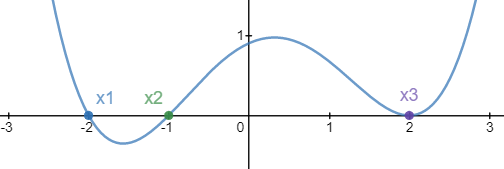
\includegraphics{roots.png}\\
			тут например $x1$ и $x2$ простые корни, а $x3$ кратный.
			\subsection{Обусловленность задачи нахождения корня}
			Для простых корней обусловенность хорошая, но чем меньше тангенс угла наклона, тем она хуже. Для кратных корней обусловленность плохая, и чем выше кратность, тем хуже.\\
			Пусть у нас есть функция $f$ определенная в окрестности нашего корня и мы хотим определить корень.\\
			Кроме того, будем пологать, что в малой окрестности корня выполняется неравенство:\\
			$|f(x)-f^{*}(x)|<\overline{\raisebox{3mm}{}\Delta}(f^{*})$\\
			\subsubsection{Интервал неопределенности}
			Заметим, что если функция f непрерывна, то\\
			$\exists U_{\overline{\upvarepsilon}}(\overline{x}): \overline{\upvarepsilon}>0$\\
			для которой выполняется\\
			\begin{equation}\label{eq:uppervalue}
			|f(x)|<\overline{\raisebox{3mm}{}\Delta}(f^{*})
			\end{equation}
			при этом в этой окрестнсоти знак $f^{*}(x)$ не обязательно должен совпадать с f(x), а значит невозможно определить какой именно $x$ является корнем. Этот интервал называется интервалом неопределенности. 
			\subsubsection{Оценка $\overline{\upvarepsilon}$}
			Пусть $\overline{x}$ - простой корень, тогда для значений близких к корню верно следующее:\\
			$f(x)\approx f(\overline{x})+f'(\overline{x})(x-\overline{x})=f'(\overline{x})(x-\overline{x})$\\
			В таком случае неравенство $\eqref{eq:uppervalue}$ примет вид\\
			$|f'(\overline{x})(x-\overline{x})| \lesssim \overline{\raisebox{3mm}{}\Delta}(f^{*})$\\
			откуда получим\\
			$\overline{x} - \frac{\overline{\raisebox{3mm}{}\Delta}(f^{*})}{|f'(\overline{x})|}
			\lesssim x \lesssim 
			\overline{x} + \frac{\overline{\raisebox{3mm}{}\Delta}(f^{*})}{|f'(\overline{x})|}
			$
			C учетом того, что\\ 
			$x\in (\overline{x} - \overline{\upvarepsilon},\ \overline{x} + \overline{\upvarepsilon})$\\
			получим\\
			$\overline{\upvarepsilon} \lesssim v_{\Delta}*\overline{\raisebox{3mm}{}\Delta}(f^{*})$\\
			$v_{\Delta} = \frac{1}{|f'(\overline{x})|}$ - в нашей задаче играеть роль абсолютного числа обусловенности. Соответственно при уменьшении $|f'(\overline{x})|$ увеличивается число обусловленности, а значит увеличивается погрешность.\\
			Для кратных корней формула для $\overline{\upvarepsilon}$ не верна, но можно разложить $f$ в ряд тейлора и получить следующее число обусловленности\\ $\overline{\raisebox{3mm}{}\Delta}(f^{*})^{\frac{-1}{m}}$
		%7
		\section{Методы половинного деления и дихотомии решения НАУ.}
			\begin{verbatim}
            solution(f, l, r)
                if !stop() then    #критерий остановки
                    #можно вернуть любое значение из [l, r] 
                    return l    
                m = (l + r) / 2
                if f(l) * f(m) <= 0 then
                    return solution(f, l, m)
                elseif f(m) * f(r) <= 0 then
                    return solution(f, m, r)
                else bad_range()
			\end{verbatim}
		%8
		\section{Метод простых итераций решения НАУ.}
            Представим нашу функцию $f$ в виде $x = g(x)$.
            \begin{verbatim}
            solution(g, x0)
                prev_x = x0
                while !stop()    #критерий остановки
                    cur_x = g(prev_x)
                    dif = abs(cur_x - prev_x)
                return cur_x 
            \end{verbatim}
		%9
		\section{Метод Ньютона решения НАУ и его модификации.}
            Пусть мы знаем производную нашей функции $f$.
		    \\ \\ %!!!!!!!!!!!!!!!!!!!!!!
            \begin{verbatim}
                solution(f, x0)
                    while stop()    #критерий остановки
                        #найдем производную нашей функции 
                        f'(x) = derivative(f)    
                        #касательная к f в точке x0
                        tangent(x) = f(x0) + f'(x0)*(x - x0)
                        #найдем точку пересечения нашей линии о осью Ox    
                        new_x = resolve(tangent = 0) 
                        x0 = new_x
                    return x0;                    
            \end{verbatim}
		%10
		\section{Понятие нормы векторов и матриц. Ассоциированная норма матрицы и ее свойства.}
            \subsection{Нормой вектора.}
            Нормой вектора называется отображение удовлетворяющее следующим свойствам:
            \begin{enumerate}
                \item{$\left\|x\right\| \geq 0$, при этом $\left\|x\right\| = 0$ только если x=0}
                \item{$\left\|ax\right\|=|a|\left\|x\right\|$, где $a$ - число}
                \item{$\left\|x+y\right\| \leq \left\|x\right\|+\left\|y\right\|$ }
            \end{enumerate}			
            В численных методах используются следующие нормы:\\
            $\left\|x\right\|_p = (\sum_{i = 1}^{m}|x_i|^p)^\frac{1}{p}$\\
            где $p \geq 1$, чаще $p = 1$ или $2$.\\ \\
            $\left\|x\right\|_p = \max|x_i|$\\
            где $1\leq i \leq m$
            \subsection{Погрешности нормы вектора.}
            $\Delta(x^{*}) = \left\|x-x^{*}\right\|$\\
            $\delta(x^{*}) = \frac{\left\|x-x^{*}\right\|}{\left\|x\right\|}$\\
            \subsection{Норма матрицы.}
            $\left\|A\right\| = max \frac{\left\|A_x\right\|}{\left\|x\right\|}$
		%11
		\section{Обусловленность задачи решения систем линейных алгебраических уравнений (СЛАУ). Стандартное число обусловленности и его свойства.}
			TODO
			
		%12
		\section{Прямые методы решения СЛАУ. Метод Гаусса и его особенности.}
			TODO
			
		%13
		\section{LU-разложение матриц.}
			TODO
			
		%14
		\section{Метод Холецкого решения СЛАУ с симметричной положительно определенной матрицей.}
			TODO
			
		%15
		\section{Метод прогонки решения СЛАУ с трехдиагональной матрицей.}
			TODO
			
		%16
		\section{Итерационные методы решения СЛАУ. Метод простых итераций (Якоби).}
			TODO
			
		%17
		\section{Методы Зейделя и последовательной релаксации решения СЛАУ.}
			TODO
			
		%18
		\section{Понятие о методах спуска решения СЛАУ. Выбор направлений и шагов спуска.}
			TODO
			
		%19
		\section{Методы покоординатного и наискорейшего спуска решения СЛАУ. Методы сопряженных направлений и градиентов.}
			TODO
			
		%20
		\section{Методы решения систем нелинейных алгебраических уравнений (обзор).}
			TODO
			
		%21
		\section{Численное нахождение собственных чисел и векторов матриц. Преобразование подобия и его свойства.}
			TODO
			
		%22
		\section{Локализация собственных чисел. Теоремы Гершгорина.}
			TODO
			
		%23
		\section{Метод Рэлея для нахождения «первого» собственного числа и вектора.}
			TODO
			
		%24
		\section{Метод вращений решения СЛАУ. QR-разложение матриц.}
			TODO
			
		%25
		\section{Метод QR-разложения для нахождения всех собственных чисел матриц.}
			TODO
			
		%26
		\section{Метод обратных итераций для нахождения всех собственных векторов матриц.}
			TODO
			
		%27
		\section{Интерполяция функций одной переменной. Интерполяционный полином в формах Лагранжа и Ньютона-Котеса.}
			TODO
			
		%28
		\section{Понятие о стратегии интерполяции. Теоремы Фабера и Чебышева о стратегии интерполяции. Универсальная стратегия интерполяции Чебышева.}
			TODO
			
		%29
		\section{Интерполяция сплайнами. Степень гладкости и дефект сплайна. Типовые сплайны третьего порядка. Физическая интерпретация сплайнов.}
			TODO
			
		%30
		\section{Аппроксимация функций одной переменной. Метод наименьших квадратов.}
			TODO
			
\end {document}
